\section{Story Diagrams} \label{sec:StoryDiagrams}

\subsection{Applications of Story Diagrams (Dietrich)}
2 worlds: with and without methods\ldots

\subsection{General composition of Story
Diagrams}\label{sec:StoryDiagrams:composition}
\begin{itemize}
  \item Based on UML 1.5 activity diagrams
  \item Grammar for story diagrams (based on grammar in diploma thesis of Thomas Klein (1999))
\end{itemize}

\subsection{Story Diagram Calls}

Story Diagram Calls are special nodes in a story diagram which are used to invoke other story diagrams. Similar to method calls, this reduces redundancy and promotes reuse.

As described in the previous sections, a story diagram can have an arbitrary number of in and out parameters. When calling a story diagram, concrete arguments have to be assigned to the in parameters. Consequently, if an object variable named n is bound somewhere in the story diagram, the identifier n can be used to pass this object variable as an argument to a call. Similarly, if the called story diagram has out parameters, those can be bound to object variables that use the same name.

In contrast to QVT \cite{QVT}, we do not explicitly model inout parameters. Instead, we allow the same objects which are passed as in parameters to be also returned as out-parameters.

An example of a story diagram call is shown in Figure~\ref{fig:call}.

\begin{figure}[htb]
\begin{center}
  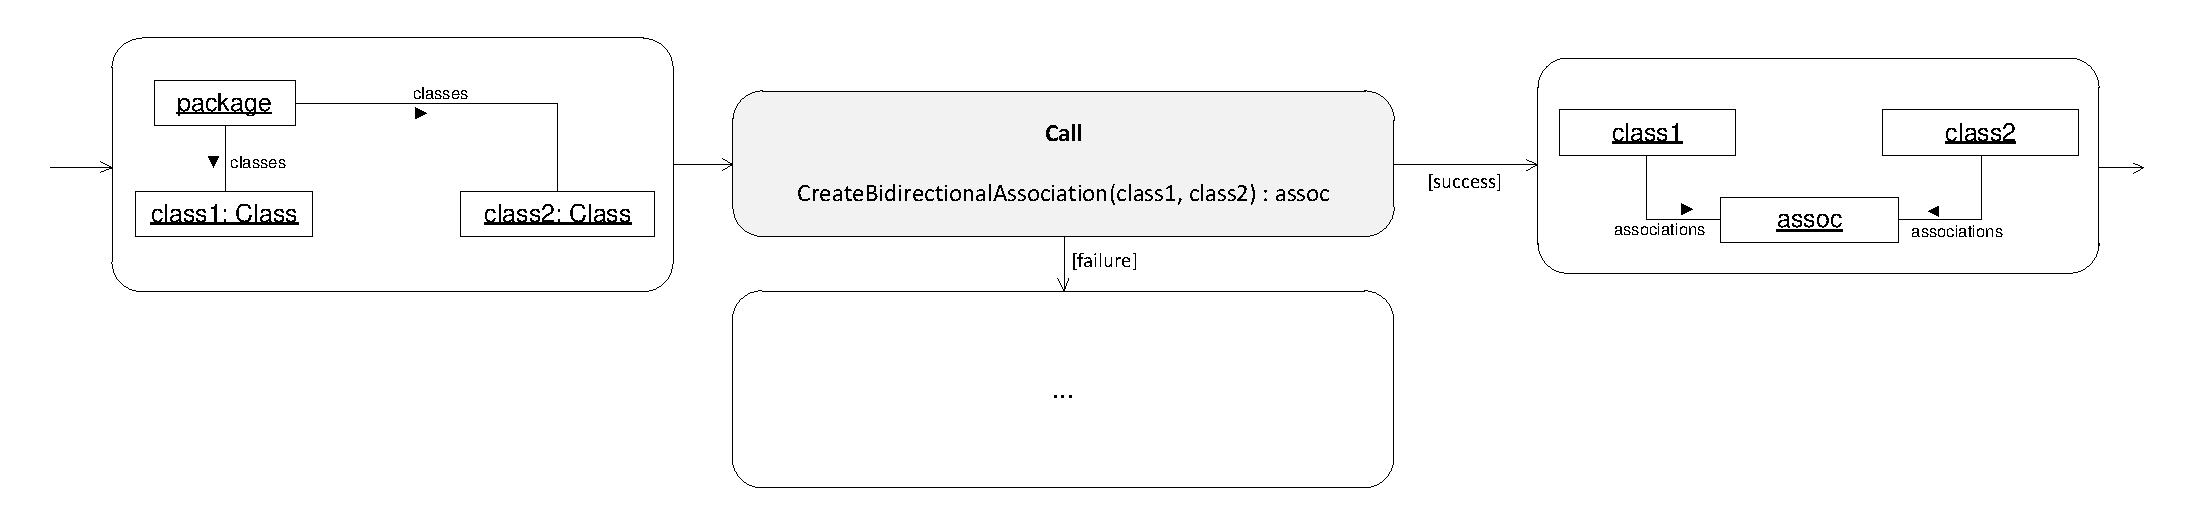
\includegraphics[width=\textwidth]{figures/StoryDiagramCall}
  \caption{Example of a story diagram call}
  \label{fig:call}
\end{center}
\end{figure}

The first story pattern in Figure~\ref{fig:call}, shows the bound object variable \fe{package}. Two new object variables \fe{class1} and \fe{class2} are bound in that pattern. The next node with the grey background is a story diagram call which is also signified by its label. Beneath the label, the name of the called story diagram is given, in this case \fe{CreateBidirectionalAssociation}. Assume that the called story diagram has two in parameters of the type \fe{Class} and one out parameter of the type \fe{Association}. The two classes that were bound in the first story pattern, \fe{class1} and \fe{class2} are passed to the call as arguments.
The result of the call is bound to the object variable \fe{assoc}. The type of this variable is determined by the out parameter type, i.e., in this case the type Association.

If a story diagram has no out parameters, the colon and the out parameters names after the parentheses are omitted (see Figure \ref{fig:SDRemoveInterfaceViolation} for an example).

%Issues for future versions:
% method calls
% polymorphic calls